%%%% ijcai19-multiauthor.tex

\typeout{IJCAI-19 Multiple authors example}

% These are the instructions for authors for IJCAI-19.

\documentclass{article}
\pdfpagewidth=8.5in
\pdfpageheight=11in
% The file ijcai19.sty is NOT the same than previous years'
\usepackage{ijcai19}

% Use the postscript times font!
\usepackage{times}
\usepackage{soul}
\usepackage{url}
\usepackage[hidelinks]{hyperref}
\usepackage[utf8]{inputenc}
\usepackage[small]{caption}
\usepackage{graphicx}
\usepackage{amsmath}
\usepackage{booktabs}
\usepackage{tikz}
\usepackage{tikz-uml}

\urlstyle{same}

% the following package is optional:
%\usepackage{latexsym} 

% Following comment is from ijcai97-submit.tex:
% The preparation of these files was supported by Schlumberger Palo Alto
% Research, AT\&T Bell Laboratories, and Morgan Kaufmann Publishers.
% Shirley Jowell, of Morgan Kaufmann Publishers, and Peter F.
% Patel-Schneider, of AT\&T Bell Laboratories collaborated on their
% preparation.

% These instructions can be modified and used in other conferences as long
% as credit to the authors and supporting agencies is retained, this notice
% is not changed, and further modification or reuse is not restricted.
% Neither Shirley Jowell nor Peter F. Patel-Schneider can be listed as
% contacts for providing assistance without their prior permission.

% To use for other conferences, change references to files and the
% conference appropriate and use other authors, contacts, publishers, and
% organizations.
% Also change the deadline and address for returning papers and the length and
% page charge instructions.
% Put where the files are available in the appropriate places.

\title{Hintikka's World: scalable higher-order knowledge}

\author{
Tristan Charrier$^1$\footnote{Contact Author}\and
Sébastien Gamblin$^2$\and
Alexandre Niveau$^{2,3}$\And
François Schwarzentruber$^4$\\
\affiliations
$^1$First Affiliation\\
$^2$Second Affiliation\\
$^3$Third Affiliation\\
$^4$Fourth Affiliation\\
\emails
\{first, second\}@example.com,
third@other.example.com,
fourth@example.com
}

\begin{document}
\newcommand{\mettel}{\textsf{MetTeL2}\xspace}

\maketitle

\begin{abstract}
	\emph{Hintikka's World} is a tool that shows how artificial agents can reason about higher-order knowledge (agent $a$ knows that agent $b$ knows that...).
	In this demonstration paper, we present symbolic models  that enables to implement in  \emph{Hintikka's World} large examples such as real card games. 
\end{abstract}



\section{Introduction}
The current trend is to construct programs that play games with imperfect information, for instance Hanabi \cite{DBLP:journals/corr/abs-1902-00506}, but also video games such as Starcraft 2 \cite{DBLP:conf/ijcai/HuLLPX18}. An important ingredient is to reason about higher-order knowledge (an agent knows that another agents knows that...). In these systems, epistemic logic and its dynamic extension, Dynamic epistemic logic (\cite{baltag1998logic}, \cite{DitmarschvdHoekKooi}) may offer formal tools for providing explanations in such AI programs. needs to be understood is relevant in AI, especially in strategic reasoning \cite{DBLP:journals/ijgt/Aumann99}.

The only pedagogical tool we are aware of that explains such models is \emph{Hintikka's world} and was presented at ECAI-IJCAI 2018 \cite{DBLP:conf/ijcai/Schwarzentruber18}. 
\emph{Hintikka's world} is a proof of concept of a graphical user interface that represent Kripke models by  comic strips, as shown in Figure \ref{figure:gui}. It enables to explore mental states of agents. The tool is available at the following address:
\url{http://hintikkasworld.irisa.fr/}. 


Kripke models are graphs, represented explicitly in memory in the first version of the tool. Explicit models are useful to learn how dynamic epistemic logic works by means of toy examples: muddy children, Sally and Anne  \cite{wimmer1983beliefs}, etc.  However, in real card games, such as Hanabi, there are an exponential number of possible configurations of cards. For instance Hanabi has 50 cards total and each player has 4 cards and the order of the cards is important. Therefore with 4 players, the initial Kripke model features $50 \times 49 \times 48 \times \dots \times 38$ configurations, that is $2.2 \times 10^{21}$. Thus, it is impossible to represent explicitly the full graph in memory:  the first version of Hintikka's world does not \emph{scale}. 

That is why, in this demonstration, we propose to represent Kripke models symbolically by using the approach in \cite{DBLP:conf/atal/CharrierS17} and \cite{DBLP:conf/aiml/CharrierS18}. The implementation relies on Binary Decision Diagrams (BDDs) \cite{} as it was done in the tool DEMO\footnote{The current implementation does not rely on DEMO since their work is not well-suited for a web application.}  \cite{DBLP:conf/lori/BenthemEGS15}. 






\begin{figure}
	\begin{center}
		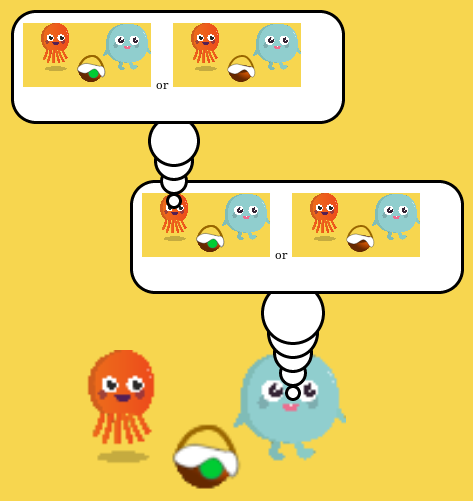
\includegraphics[width=4cm]{screenshot.png} TODO ajouter le modèle de Kripke
	\end{center}
	\caption{Graphical user interface of \emph{Hintikka's world}.\label{figure:gui}}
\end{figure}


\section{Demonstration Outline}
\label{section:demonstration}

In the demonstration we run through a game of (a variant of) Hanabi. 
In Hanabi, each agent has cards with a color and a
number, but cannot see his/her own hand.
At each turn, in \emph{Hintikka's World}, the user can play the role of one of the agents: he/she can either give the information to some other agent about a number or a color, or play a card. The goal is to play the cards in increasing order for each color.
During the process, the system keeps track on the knowledge of the agents.
More precisely, the system shows the real world (the real distribution of the cards). When the user clicks on an agent, the system displays a \emph{sampling} of some possible worlds for that agent (i.e., some distributions of cards he/she still considers as possible at this stage of the game). The agents also reason about knowledge of other agents, as shown in Figure~\ref{figure:guihanabi} (two levels of knowledge are shown).
%
%
%% expliquer la démo. Je me suis peut etre trompé sur le nombre de cartes ici et si on gère les jetons pour les infos il faut le mettre dans le paragraphe.
% Alex: pas grave au pire. on dit qu'on peut faire ça ou ça, c'est pas _forcément_ exclusif.
%


\begin{figure}
	\begin{center}
		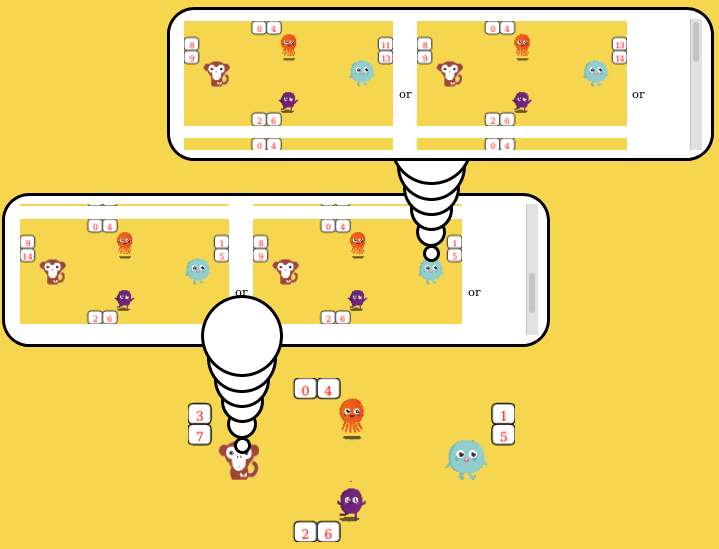
\includegraphics[width=4cm]{images/HW_screenshot_hanabi.png}
	\end{center}
\vspace{-3mm}
	\caption{Screenshot of Hanabi in \emph{Hintikka's World}.\label{figure:guihanabi}}
\end{figure}
%%\newpage

Note that in this demonstration, in order to explain models of DEL, the tool still presents examples that rely on explicit models, such as ``Sally and Anne'', ``Muddy Children'', ``Consecutive Numbers'', etc.



\section{Symbolic models}
\label{section:symbolicmodels}
In our tool, we definitely emphasize on the use of model checking over theorem proving, as advocated in \cite{DBLP:conf/kr/HalpernV91}. More precisely, we use the same ideas than in symbolic model checking, as defined for temporal logics \cite{DBLP:conf/lics/BurchCMDH90}, adapted to DEL, as explained in \cite{DBLP:conf/atal/CharrierS17} and \cite{DBLP:conf/aiml/CharrierS18}. Our model checking procedure relies now on symbolic Kripke models, aimed at representing succinctly so-called pointed Kripke models. A pointed Kripke model is a graph whose nodes are \emph{possible worlds}, edges are labeled by agents and an edge $w \rightarrow^a u$ means that agent $a$ considers world $u$ as possible in world $w$. Each world $w$ is equipped with a valuation telling which atomic propositions is true in $w$. A special world is called the pointed world and represents the true situation, while the other possible worlds are worlds imagined by the agents.
The tool shows that graph in the right-part of the screen (in the example of Figure~\ref{figure:gui}, the Kripke model has two possible worlds, $w$ and $u$, $p$ is true in $w$ but not in $u$, and $\rightarrow_a$ is given in red and $\rightarrow_b$ in blue). 


\newcommand{\succinctsetworlds}{\chi}
\newcommand{\succinctrelation}[1]{\pi_{#1}}
 A symbolic model gives a Boolean formula $\succinctsetworlds(\vec x)$ that succinctly  describes the set of possible worlds: a world is a valuation over Boolean variables $\vec x$ satisfing $\succinctsetworlds(\vec x)$. It also gives, for each agent $a$, a Boolean formula $\succinctrelation a(\vec x, \vec x')$ that tells whether there is an edge labeled by agent $a$ from a world described by a valuation over $\vec x$ and  a world described by a valuation over $\vec x'$. All these Boolean formula are then classically converted in BDDs.%is in a description of the model in a more succinct language. Such representations already exist for other formalisms, such as boolean circuits for searching for Hamiltonian paths in graphs \cite{papadimitriou2003computational}, or BDDs in symbolic model checking .

%In the demonstration we use the symbolic description of \cite{DBLP:conf/aiml/CharrierS18} for dynamic epistemic logic \footnote{Which is actually a rewriting of the description of \cite{DBLP:conf/atal/CharrierS17}}, and use the reduction to first-order logic of \cite{DBLP:conf/tableaux/CharrierPS17} to implement this approach with BDDs.

Typically, for Hanabi, $\succinctsetworlds(\vec x)$ tells that $\vec x$ describes an initial possible configuration. Formula $\succinctrelation a(\vec x, \vec x')$ tells that the agents diferent from $a$ have the same card in $\vec x$ and $\vec x'$ (it models the fact that agent $a$ sees the cards of the other players).
%Take for instance any card game. The initial model is described by BDDs for the following boolean formulas: formula $\chi_W$  whose valuations are the possible configurations and formula $\chi_R$ to describe which configurations agents do not distinguish. The formula $\chi_W$ actually describes legal configurations according to the rules of the game, and $\chi_W$ reflect the fact that agents do not see the hand of other agents, so they may imagine as possible any possible dealing.

Dynamic epistemic logic also provides so-called \emph{event models} for describing actions (public announcements, public actions, private announcements/actions, etc.). The reader may refer to the textbook on DEL \cite{DitmarschvdHoekKooi} and to \cite{DBLP:conf/atal/CharrierS17} for symbolic event models, that we do not detail here.







\section{System Description}
\label{section:architecture}

Whereas the first version was written in Javascript In order to ease the development, the new version is written in TypeScript and Angular 7.

\subsection{Binary decision diagrams}

As shown in \cite{DBLP:conf/atal/CharrierS17}, the symbolic model checking of DEL is PSPACE-complete, thus is critical. We manipulate set of worlds, and relations by means of Binary decision diagrams. To this aim, we wrote a wrap-up in C of the library CUDD (Colorado University Decision Diagram Package) \cite{DBLP:journals/sttt/Somenzi01}, that produces a Web Assembly library and a Javascript module.

In order to show possible worlds for a given agent $a$ in some world $w$, we first construct the BDD of $\succinctrelation a(descr(w), \vec x')$ where $descr(w)$ are the Boolean values of $\vec x$ corresponding to world $w$. We then count the number of possible valuations $\vec x'$ than makes for randomly values for $\vec x'$ that makes $\succinctrelation a(descr(w), \vec x')$ true (BDDs are convenient for counting, see TODO). If the number of such valuations is small, we show all the possible worlds, otherwise we randomly generate valuations for $\vec x'$ that makes $\succinctrelation a(descr(w), \vec x')$ true (we randomly select a branch that leads to the true-leaf in the BDD of $\succinctrelation a(descr(w), \vec x')$).

\subsection{Class Architecture}

Figure \ref{figure:architecture} shows the new architecture of \emph{Hintikka's world}. \texttt{EpistemicModel} is an abstract class used by the graphical user interface (GUI), that is independent from the current runnin example (muddy children, Sally and Anne, Hanabi, etc.) but more interestingly independent from the representation of the epistemic model itself. In particular, an epistemic model can be an \texttt{ExplicitEpistemicModel} (a graph) or a \texttt{SymbolicEpistemicModel} that relies on BDDs, depending on the examples: it suffices to implement the method \texttt{draw} of a class that inherits from class \texttt{World}.


\subsection{Adding new examples}

The system is easy to use to provide new examples. Explicit epistemic models are directly described (set of nodes and of edges). Symbolic epistemic models are described by a Boolean formula $\succinctsetworlds$, or Boolean formulas for $\succinctrelation{a}$. The system provides a way to easily describe how worlds are displayed in the comic strips.

\begin{figure}
	\begin{center}
		\scalebox{0.6}{
			\begin{tikzpicture}[scale=0.75]
			
			\umlclass[x=0,y=2]{EpistemicModel}{
				
			}{}
			
			\umlclass[x=-6,y=2]{Graph}{
			}{
			}
			
%			\umlclass[x=-2,y=-2.5]{World}{
%			}{
%			}

	\umlclass[x=8,y=2]{BDD}{
}{
}
			
			\umlclass[x=-3,y=-0]{ExplicitEpistemicModel}{
			}{
			}
			
			\umlclass[x=4,y=-2.4]{Hanabi}{
			}{
			}
			
			\umlclass[x=-3,y=-2.4]{SallyAndAnne}{
			}{
			}
			
			\umlclass[x=4,y=-0]{SymbolicEpistemicModel}{
			}{
			}
			
			
		%	\umlassoc[geometry=--, arg1=, mult1=1, align1=right, arg2=, mult2=*, align2=left]{GUI}{EpistemicModel}
		%	\umlassoc[geometry=--, arg1=, mult1=*, arg2=, mult2=1]{EpistemicModel}{World}
			\umlassoc[geometry=--, arg1=, mult1=, arg2=, mult2=1]{ExplicitEpistemicModel}{SallyAndAnne}
			\umlassoc[geometry=--, arg1=, mult1=, arg2=, mult2=1]{SymbolicEpistemicModel}{Hanabi}
			\umlinherit[geometry=|-]{ExplicitEpistemicModel}{Graph}
			\umlinherit[geometry=|-]{SymbolicEpistemicModel}{EpistemicModel}
			\umlinherit[geometry=|-]{ExplicitEpistemicModel}{EpistemicModel}
			\umlassoc[geometry=-|, arg1=, mult1=*, arg2=, mult2=]{SymbolicEpistemicModel}{BDD}			

			
			%\umlunicompo[geometry=-|, arg=titi, mult=*, pos=1.7, stereo=vector]{D}{C}
			%\umlaggreg[arg=tutu, mult=1, pos=0.8, angle1=30, angle2=60, loopsize=2cm]{D}{D}
			
			\end{tikzpicture}}
		\vspace{-3mm}
	\end{center}
	\caption{New architecture of \emph{Hintikka's world}.\label{figure:architecture}}
\end{figure}

\section{Future Work}
\label{section:perspectives}

TODO implémzenter d'autres exemples etc.


TODO d'autres façons de "scaler" (parler des ATD)

TODO parler de méthodes statistiques pour générer des mondes possibles










\newpage



\bibliographystyle{named}
\bibliography{biblio}




\end{document}

